%%%%%%%%%%% DTI report %%%%%%%%%%%
\documentclass[a4paper,11pt,oneside]{DTI}

% *************** Load packages ***************
\usepackage[T1]{fontenc}
\usepackage[italian]{babel}
\usepackage{graphicx}
\usepackage{url}
\usepackage{subfigure}
\usepackage{makeidx}
\usepackage[utf8]{inputenc}
\usepackage{booktabs}
\usepackage[colorlinks]{hyperref}
\usepackage{amsmath}
\usepackage{amsfonts}
\usepackage{amssymb}
\usepackage{listings}

\title{Traveling Salesman Problem}
\subTitle{19\ap{a} Coppa di Algoritmi} 
\author{Alessandro Bianchi}

\date{\today}

\lstset{language=bash}

% Crea un capitolo senza numerazione che per� appare nell'indice %
\newcommand{\problemchapter}[1]{%
  \chapter*{#1}%
  \addcontentsline{toc}{chapter}{#1}%
\markright{#1}{}}

%*****************************************************************

% Numerazione delle appendici secondo norma %
\addto\appendix{\renewcommand{\thesection}{\Alph{section}} 
\renewcommand{\thesubsection}{\thesection.\arabic{subsection}}}
%*****************************************************************

\makeindex % Crea l'indice analitico, se è necessario scommentarlo
\begin{document}
\maketitle
\frontmatter
\newpage
\mainmatter
% *************** Main matter ***************

%\chapter*{Problema}
\label{cha_problema}

Il problema del commesso viaggiatore consiste nella ricerca del ciclo hamiltoniano più breve all'interno di un grafo pesato completo. Questo tipo di problema appartiene alla classe dei problemi \emph{NP-Completi}. In Figura~\ref{fig_eil76} è mostrato uno dei problemi TSP con soluzione, sottoinsieme dei problemi NP.

\begin{figure}
  \centering
  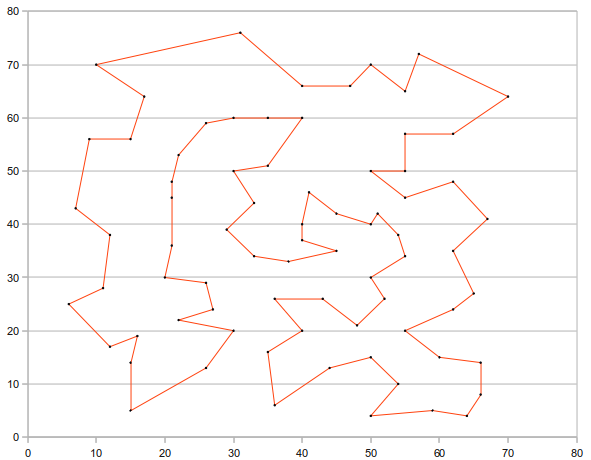
\includegraphics[width=10.0cm]{immagini/eil76.png}
  \caption{Eil76, problema di TSP da 76 città\label{fig_eil76}}
\end{figure}

Il compito assegnato è di generare una soluzione ammissibile e quanto più possibile vicina a quella ottimale (ovvero la migliore) in 3 minuti di esecuzione del programma. Il programma deve poter lavorare su 10 problemi diversi:
\begin{itemize}
  \item \emph{ch130};
  \item \emph{d198};
  \item \emph{eil76};
  \item \emph{fl1577};
  \item \emph{kroA100};
  \item \emph{lin318};
  \item \emph{pcb442};
  \item \emph{pr439};
  \item \emph{rat783};
  \item \emph{u1060}.
\end{itemize}



\chapter*{Problema}
\label{cha_problema}

Il problema è il Traveling Salesman Problem (TSP): dato un insieme di città trovare il percorso più corto che le visiti tutte senza passare due volte dalla stessa città.\\

Per il progetto, è stata richiesta l'implementazione di uno o più algoritmi di ricerca (vedi capitolo "Soluzioni Implementate").

%\chapter*{Soluzioni implementate}
\label{cha_soluzioni}

\section*{Algoritmo costruttivo}
\label{sec_costruttivo}
L'algoritmo costruttivo ha il compito di generare una prima soluzione ammissibile. La mia scelta si è volta verso un algoritmo \emph{random} e \emph{farthest insertion}. \\
\noindent 

\section*{Algoritmi di ottimizzazione locale}
\label{sec_ottimizzazione}
Non implementato.

\section*{Algoritmi meta-euristici}
\label{sec_metaeuristici}
Non implementato.

\chapter*{Soluzioni implementate}
\label{cha_soluzioni}

\section*{Algoritmi}
\subsection*{Algoritmi meta-euristici}
\label{sec_metaeuristici}
L'algoritmo metaeuristico implementato è l'\textbf{Ant Colony Optimization (ACO)}. L'algoritmo prevede un certo numero di formiche che, spostandosi tra le varie città attraverso due possibilità (\textit{exploration} o \textit{exploitation}), lasciano lungo la via del feromone che le formiche successive utilizzeranno per migliorare il risultato di volta in volta.

\subsection*{Algoritmo costruttivo}
\label{sec_costruttivo}

L'algoritmo di tipo costruttivo scelto per l'implementazione è il \textbf{nearest neighbor}. Grazie a questo è possibile generare in maniera rapida una soluzione ammissibile del problema. \'E inoltre utilizzato per calcolare il feromone iniziale nell'algoritmo \textit{ACO}.

\subsection*{Algoritmo di ottimizzazione locale}
\label{sec_ottimizzazione}
L'algoritmo di ottimizzazione scelto è il 2-OPT. 2-OPT è utilizzato per ottimizzare il percorso ottenuto dalle formiche dell'\textit{ACO}.


\section*{Altre funzionalità}
\'E possibile disegnare il percorso di ogni tour utilizzando i uno tra i metodi \textit{getVisualTour()} e \textit{betterDraw()} presenti nella classe Tour. Per l'esecuzione dei test, il codice relativo alla visualizzazione dei percorsi è commentato.


\chapter*{Risultati}
\label{cha_risultati}

Nella Tabella~\ref{tab_parametri} sono riportati i parametri utilizzati per l'esecuzione dell'ACO.\\
Nella Tabella~\ref{tab_risultati} sono mostrati i risultati ottenuti per ogni problema.\\

\begin{table}[htb]
  \caption{Parametri utilizzati per ogni problema}
  \label{tab_parametri}
  \centering
\begin{tabular}{lrrrrrrr}
  \toprule
  Problema		&	Alpha		&	Beta	&	Exploitation &	Formiche &  Iterazioni  &	Seed 1		&	Seed 2\\
  \midrule
  ch130			&	0.1			&	2		&	0.9	  & 10 & 150	&   10000000	&	0\\
  d198			&	0.1			&	2		&	0.9   & 10 & 350 &	10000000	&	0	\\
  eil76			&	0.1		    &	2		&	0.9   & 10 & 150 &	10000000	&	0	\\
  fl1577		&	0.1			&	2		&	0.9   & 3  & 44	&	10000000	&	0	\\
  kroA100		&	0.1			&	2		&	0.9   & 10 & 150	&   10000000	&	0	\\
  lin318		&	0.1			&	2		&	0.9   & 10 & 350	&	10000000	&	0	\\
  pcb442		&	0.1			&	2		&	0.9   & 10 & 350	&	10000000	&	0	\\
  pr439			&	0.1			&	2		&	0.9   & 10 & 350	&	10000000	&	0	\\
  rat783		&	0.1			&	2		&	0.9   & 10 & 67	&	10000000	&	0	\\
  u1060			&	0.1			&	2		&	0.9   & 10 & 23	&	10000000	&	0	\\
  \midrule
  %media			&			&			&	1635.11\% 	&			\\
  %\bottomrule
\end{tabular}
\end{table}

\begin{table}[htb]
  \caption{Soluzioni calcolate per ogni soluzione}
  \label{tab_risultati}
  \centering
\begin{tabular}{lrrr}
  \toprule
  Problema		&	Ottimo		&	Risultato	&	Errore		\\
  \midrule
  ch130			&	6110		&	6110		&	0.0\%	  \\
  d198			&	15780		&	15780		&	0.0\%	  \\
  eil76			&	538		    &	538		   &	0.0\%	  \\
  fl1577		&	22249		&	22652		&	1,81\% \\
  kroA100		&	21282		&	21282		&	0.0\%	  \\
  lin318		&	42029		&	42091		&	0,15\% \\	
  pcb442		&	50788		&	51019		&	0,47\% \\
  pr439			&	107217		&	107271		&	0,05\% \\
  rat783		&	8806		&	8955		&	1,69\% \\
  u1060			&	224094		&	229895		&	2723.26\% \\
  \midrule
  media			&			&			&	0,676 \% 			\\
  \bottomrule
\end{tabular}
\end{table}




%\chapter*{Conclusioni}
\label{cha_conclusioni}

L'algoritmo implementato è chiaramente inefficiente: la media finale dell'errore è 1635.11\%. 
\chapter*{Conclusioni}
I risultati ottenuti, come confermato dalla media, sono piuttosto buoni: su 3 problemi gli algoritmi riescono a replicare l'ottimo e solamente due sono oltre l'1\% di errore.\\
Lavorando ancora per trovare dei parametri migliori, è sicuramente possibile cercare di ridurre ancora l'errore.\\
\end{document}
